Описание процесса определения авторства исходного кода программ в виде модели <<черного ящика>> согласно 
методологии IDEF0 представлено на рисунке~\ref{box_1:box_1}, его декомпозиция --- 
в приложении~Г.
% на рисунке~\ref{box_2:box_2}.

\begin{figure}[h!]
\center{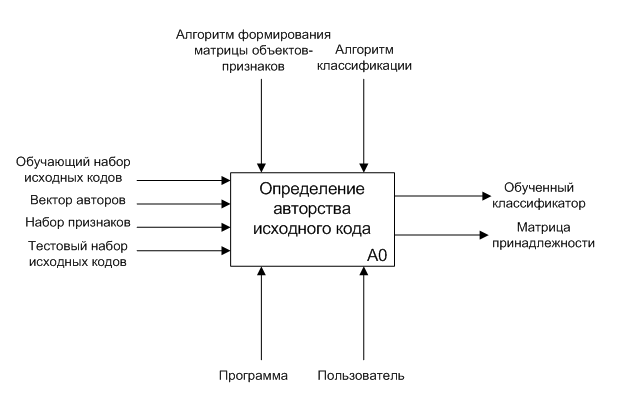
\includegraphics[width=0.8\linewidth]{box_1}}
\caption{ Модель <<черного ящика>> процесса определения авторства исходного кода по методологии IDEF0 }
\label{box_1:box_1}
\end{figure} 

% \begin{figure}[h!]
% \center{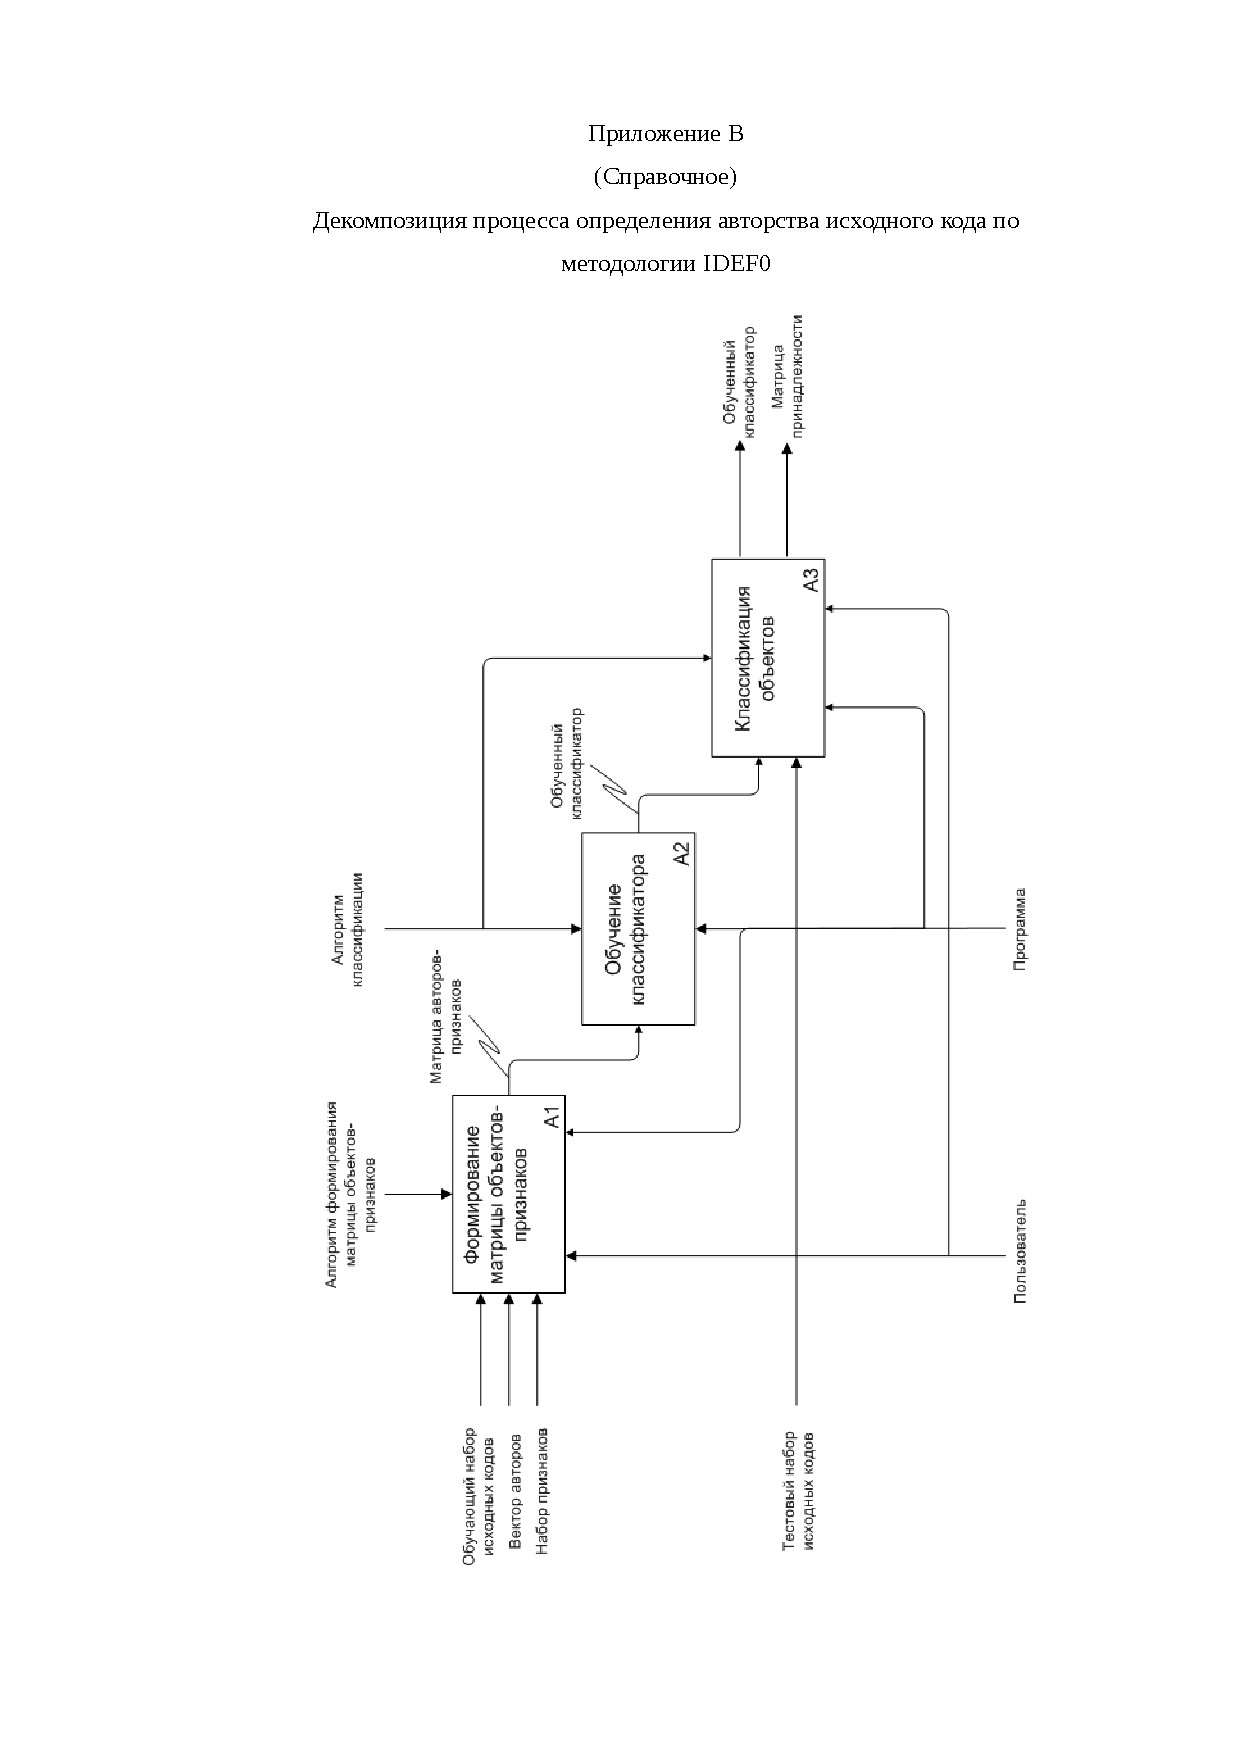
\includegraphics[width=1\linewidth]{box_2}}
% \caption{ Декомпозиция <<черного ящика>> процесса определения авторства исходного кода по методологии IDEF0 }
% \label{box_2:box_2}
% \end{figure} 
